%File: anonymous-submission-latex-2026.tex
\documentclass[letterpaper]{article} % DO NOT CHANGE THIS
\usepackage[submission]{aaai2026}  % DO NOT CHANGE THIS
\usepackage{times}  % DO NOT CHANGE THIS
\usepackage[edges]{forest}
\usepackage[edges]{forest}
\usepackage[edges]{forest}

\forestset{
  roof/.style={
    for children={no edge},
    tikz+={
      \path (.children first) coordinate (firstchild);
      \path (.children last) coordinate (lastchild);
      \draw (.south) -- (firstchild.north);
      \draw (.south) -- (lastchild.north);
      \draw (firstchild.north) -- (lastchild.north);
    }
  }
}

\usepackage{amssymb}
\DeclareUnicodeCharacter{22C6}{\ensuremath{\star}}
\usepackage{microtype}
\usepackage{listings}
\usepackage{helvet}  % DO NOT CHANGE THIS
\usepackage{courier}  % DO NOT CHANGE THIS
\usepackage[hyphens]{url}  % DO NOT CHANGE THIS
\usepackage{graphicx} % DO NOT CHANGE THIS
\urlstyle{rm} % DO NOT CHANGE THIS
\def\UrlFont{\rm}  % DO NOT CHANGE THIS
\usepackage{natbib}  % DO NOT CHANGE THIS AND DO NOT ADD ANY OPTIONS TO IT
\usepackage{caption} % DO NOT CHANGE THIS AND DO NOT ADD ANY OPTIONS TO IT
\frenchspacing  % DO NOT CHANGE THIS
\setlength{\pdfpagewidth}{8.5in} % DO NOT CHANGE THIS
\setlength{\pdfpageheight}{11in} % DO NOT CHANGE THIS
%
% These are recommended to typeset algorithms but not required. See the subsubsection on algorithms. Remove them if you don't have algorithms in your paper.
\usepackage{amsmath}
\usepackage{graphicx}
\usepackage{amssymb}
\usepackage{float}
\usepackage{algorithm}
\usepackage{algorithmic}

\newfloat{dataset}{t}{lod}
\floatname{dataset}{Dataset element}
\usepackage{tabularx}
\usepackage{booktabs}
\newcolumntype{Y}{>{\centering\arraybackslash}X} % Creates a centered 'X' column
\usepackage{comment}
\usepackage{pgfkeys}
\usepackage{tikz}
\usetikzlibrary{
  positioning,
  shapes.geometric,
  arrows.meta,
  backgrounds,
  fit
}


%
% These are are recommended to typeset listings but not required. See the subsubsection on listing. Remove this block if you don't have listings in your paper.
\usepackage{newfloat}
\usepackage{listings}
\DeclareCaptionStyle{ruled}{labelfont=normalfont,labelsep=colon,strut=off} % DO NOT CHANGE THIS
\lstset{%
	basicstyle={\footnotesize\ttfamily},% footnotesize acceptable for monospace
	numbers=left,numberstyle=\footnotesize,xleftmargin=2em,% show line numbers, remove this entire line if you don't want the numbers.
	aboveskip=0pt,belowskip=0pt,%
	showstringspaces=false,tabsize=2,breaklines=true}
\floatstyle{ruled}
\newfloat{listing}{tb}{lst}{}
\floatname{listing}{Listing}
%
% Keep the \pdfinfo as shown here. There's no need
% for you to add the /Title and /Author tags.
\pdfinfo{
/TemplateVersion (2026.1)
}

% DISALLOWED PACKAGES
% \usepackage{authblk} -- This package is specifically forbidden
% \usepackage{balance} -- This package is specifically forbidden
% \usepackage{color (if used in text)
% \usepackage{CJK} -- This package is specifically forbidden
% \usepackage{float} -- This package is specifically forbidden
% \usepackage{flushend} -- This package is specifically forbidden
% \usepackage{fontenc} -- This package is specifically forbidden
% \usepackage{fullpage} -- This package is specifically forbidden
% \usepackage{geometry} -- This package is specifically forbidden
% \usepackage{grffile} -- This package is specifically forbidden
% \usepackage{hyperref} -- This package is specifically forbidden
% \usepackage{navigator} -- This package is specifically forbidden
% (or any other package that embeds links such as navigator or hyperref)
% \indentfirst} -- This package is specifically forbidden
% \layout} -- This package is specifically forbidden
% \multicol} -- This package is specifically forbidden
% \nameref} -- This package is specifically forbidden
% \usepackage{savetrees} -- This package is specifically forbidden
% \usepackage{setspace} -- This package is specifically forbidden
% \usepackage{stfloats} -- This package is specifically forbidden
% \usepackage{tabu} -- This package is specifically forbidden
% \usepackage{titlesec} -- This package is specifically forbidden
% \usepackage{tocbibind} -- This package is specifically forbidden
% \usepackage{ulem} -- This package is specifically forbidden
% \usepackage{wrapfig} -- This package is specifically forbidden
% DISALLOWED COMMANDS
% \nocopyright -- Your paper will not be published if you use this command
% \addtolength -- This command may not be used
% \balance -- This command may not be used
% \baselinestretch -- Your paper will not be published if you use this command
% \clearpage -- No page breaks of any kind may be used for the final version of your paper
% \columnsep -- This command may not be used
% \newpage -- No page breaks of any kind may be used for the final version of your paper
% \pagebreak -- No page breaks of any kind may be used for the final version of your paperr
% \pagestyle -- This command may not be used
% \tiny -- This is not an acceptable font size.
% \vspace{- -- No negative value may be used in proximity of a caption, figure, table, section, subsection, subsubsection, or reference
% \vskip{- -- No negative value may be used to alter spacing above or below a caption, figure, table, section, subsection, subsubsection, or reference

\setcounter{secnumdepth}{2} %May be changed to 1 or 2 if section numbers are desired.

% The file aaai2026.sty is the style file for AAAI Press
% proceedings, working notes, and technical reports.
%

% Title

% Your title must be in mixed case, not sentence case.
% That means all verbs (including short verbs like be, is, using,and go),
% nouns, adverbs, adjectives should be capitalized, including both words in hyphenated terms, while
% articles, conjunctions, and prepositions are lower case unless they
% directly follow a colon or long dash
\title{Translating Natural Language to Strategic
Temporal Specifications via LLMs}
\author{
    %Authors
    % All authors must be in the same font size and format.
    Written by AAAI Press Staff\textsuperscript{\rm 1}\thanks{With help from the AAAI Publications Committee.}\\
    AAAI Style Contributions by Pater Patel Schneider,
    Sunil Issar,\\
    J. Scott Penberthy,
    George Ferguson,
    Hans Guesgen,
    Francisco Cruz\equalcontrib,
    Marc Pujol-Gonzalez\equalcontrib
}
\affiliations{
    %Afiliations
    \textsuperscript{\rm 1}Association for the Advancement of Artificial Intelligence\\
    % If you have multiple authors and multiple affiliations
    % use superscripts in text and roman font to identify them.
    % For example,

    % Sunil Issar\textsuperscript{\rm 2},
    % J. Scott Penberthy\textsuperscript{\rm 3},
    % George Ferguson\textsuperscript{\rm 4},
    % Hans Guesgen\textsuperscript{\rm 5}
    % Note that the comma should be placed after the superscript

    1101 Pennsylvania Ave, NW Suite 300\\
    Washington, DC 20004 USA\\
    % email address must be in roman text type, not monospace or sans serif
    proceedings-questions@aaai.org
%
% See more examples next
}

%Example, Single Author, ->> remove \iffalse,\fi and place them surrounding AAAI title to use it
\iffalse
\title{My Publication Title --- Single Author}
\author {
    Author Name
}
\affiliations{
    Affiliation\\
    Affiliation Line 2\\
    name@example.com
}
\fi

\iffalse
%Example, Multiple Authors, ->> remove \iffalse,\fi and place them surrounding AAAI title to use it
\title{My Publication Title --- Multiple Authors}
\author {
    % Authors
    First Author Name\textsuperscript{\rm 1},
    Second Author Name\textsuperscript{\rm 2},
    Third Author Name\textsuperscript{\rm 1}
}
\affiliations {
    % Affiliations
    \textsuperscript{\rm 1}Affiliation 1\\
    \textsuperscript{\rm 2}Affiliation 2\\
    firstAuthor@affiliation1.com, secondAuthor@affilation2.com, thirdAuthor@affiliation1.com
}
\fi


% REMOVE THIS: bibentry
% This is only needed to show inline citations in the guidelines document. You should not need it and can safely delete it.
\usepackage{bibentry}
% END REMOVE bibentry

\forestset{
  default preamble={
    for tree={
      font=\small,
      parent anchor=south,
      child anchor=north,
      align=center,
      base=top,
      where n children=0{tier=word}{},
      inner sep=2pt,
      l sep=6mm,
      s sep=4mm,
    }
  }
}

\begin{document}

\maketitle

%Absgtract ridurre di 1/3
%Intro+related works e outile devono finire a pagina 2, prima colonna
% Backgroung deve stare in una colonna e mezza. Meglio se finisce tutto fino a qui entro le prime due pagine.
%DAtaset due colenne (entro fine pagina 3)
%Framework da 6 a 4 colonne e isamo dunque a pagina 5
%Evaluation + experiments, poco meno di due pagine e siamo dunque quasi a fine pagina 7.
% quello che rimane di pagina 7 (circa mezza colonna), da distare alle conclusione future work.
% commenti generali, ridurre il font dell'environment algorithm e ridurre al minimo le immagini (usare wrapfig se necessario
%mettere in linea sintassi di ATL* e semplificare quella di ATL
%semplificare anche la notazione, per esempio per [i...j], scriverne una e richiamare le altre come caso particolare
%parlare solo di ATL* e richiamare ATL solo come caso particolare
%manovrare gli esperimenti in tabella 1 con gli ultime versioni di modelli generativi

\begin{abstract}
Rigorous formal specifications are a prerequisite for verifying Multi-Agent Systems (MAS), yet writing them is error-prone, time-consuming, and expertise-intensive---especially when requirements must capture both the strategic abilities of agents and their temporal objectives. Despite the central role of strategic logics in verification, no established methodology derives MAS specifications from natural language. We present a framework that translates natural-language descriptions of strategic requirements into well-formed ATL/ATL$^*$ formulas using Large Language Models (LLMs). Because no dataset supports supervised learning for the NL-to-ATL/ATL$^*$ translation task, we create and curate a novel dataset of $1100$ instances, hand-written and validated by domain experts. On a held-out test set, evaluated under the LLM judge that best agrees with expert annotations, in-domain fine-tuning of small open-weight models ($3$--$7$B parameters) matches strong few-shot proprietary API baselines---our best fine-tuned system reaches $0.84$ semantic accuracy, statistically on par with $0.86$ for the strongest few-shot proprietary baseline---while keeping requirements on-premises. We further find that judge reliability is inverse to generator strength: the open-weight Llama-3.3-70B tracks human verdicts most closely, whereas the strongest proprietary models are the least reliable judges, over-rejecting faithful paraphrases of the reference. To assess the practical applicability of the generated specifications, we connect our tool to an existing strategic-logics model checker, enabling non-expert users to specify strategic properties in natural language.
\end{abstract}

% Uncomment the following to link to your code, datasets, an extended version or similar.
% You must keep this block between (not within) the abstract and the main body of the paper.
% \begin{links}
%     \link{Code}{https://aaai.org/example/code}
%     \link{Datasets}{https://aaai.org/example/datasets}
%     \link{Extended version}{https://aaai.org/example/extended-version}
% \end{links}
\section{Introduction}

Formal verification of Multi-Agent Systems (MAS) requires logical formalisms capable of capturing how multiple agents interact, compete, and cooperate over time \cite{shoham2008multiagent,wooldridge2009introduction,DBLP:journals/tocl/MogaveroMPV14}. In this setting, strategic logics such as Alternating-time Temporal Logic (ATL$^\ast$) \cite{alur2002alternating} provide a natural framework for specifying what coalitions of agents can enforce, regardless of the behavior of others. This makes the logic particularly suitable for safety-critical and adversarial scenarios, where guarantees must hold even in the presence of uncontrollable or competing entities. Yet, writing correct ATL$^\ast$ specifications requires substantial expertise in formal methods, temporal logic, and game-theoretic semantics, making the construction of strategic specifications difficult to non-expert practitioners. This remains true even for ATL, the vanilla fragment of ATL$^\ast$. A major source of difficulty is that requirements are typically expressed in natural language, which is inherently ambiguous, both because its interpretation depends on context and because the same surface form may admit different structural readings \cite{saussure1916course,small2013lexical}. In formal verification, however, ambiguity cannot be tolerated: verification pipelines require well-formed formulas with precise syntax and unambiguous semantics. More generally, the gap between linguistic expression and logical form has long motivated the view that the surface grammar of a sentence may fail to make its underlying formal structure explicit \cite{frege1892sense,russell1905denoting,Russell1919-RUSTPO-65}. In the context of strategic reasoning, this mismatch becomes especially critical, since ambiguities may affect coalition attribution, temporal scope, and the intended interpretation of alternative strategic outcomes \cite{kulkarni2025dynamic}. These issues are further amplified when natural-language requirements are processed by Large Language Models (LLMs). Besides inheriting the intrinsic ambiguity of natural language, LLM inputs may also be under-specified or contain irrelevant task-related details, both of which can lead to multiple plausible formalizations of the same request. This is particularly problematic in the strategic setting, where even small differences in interpretation may produce logically distinct ATL or ATL$^\ast$ formulas with substantially different verification outcomes.

Recent advances in LLMs have generated growing interest in the automatic translation of natural-language requirements into formal specifications. Existing work, however, has focused predominantly on single-agent or purely temporal formalisms, such as Linear Temporal Logic (LTL) \cite{pnueli1977temporal}, Signal Temporal Logic (STL) \cite{maler2004monitoring}, and Computation Tree Logic (CTL) \cite{clarke1981design}. By contrast, the strategic setting of MAS remains largely unexplored. To the best of our knowledge, there is currently no established trained LLM, nor any publicly available dataset, specifically designed to support the translation of natural-language requirements into ATL or ATL$^\ast$ specifications.

\paragraph{Our Contributions.}
We introduce an open-weight, open-source LLM framework for translating natural-language requirements involving strategic reasoning into well-formed ATL/ATL$^\ast$ formulas. Our contributions are:

\begin{itemize}
    \item \textbf{First expert-authored NL-to-ATL/ATL$^\ast$ dataset.}
    We release, to the best of our knowledge, the first benchmark for translating natural-language requirements into ATL/ATL$^\ast$ formulae: 1100 instances hand-written by three domain experts and covering coalitional ability, adversarial outcomes, temporal objectives, and five ambiguity families: right dislocation, left dislocation, VP ellipsis, Right Node Raising, and quantifier scope. The dataset is approximately balanced across ATL/ATL$^\ast$ temporal operators and ambiguity types, and uses diverse realizations to avoid surface-template bias. 

    \item \textbf{Hybrid open-weight translation framework.}
    We propose an LLM-based NL-to-ATL/ATL$^\ast$ translation framework supporting both Azure OpenAI inference and private local deployment with open-weight models, enabling cloud-scale experimentation and privacy-sensitive industrial use.

    \item \textbf{Fine-tuning and judge reliability.}
    We fine-tune open-weight models on our dataset and compare them with strong few-shot proprietary baselines. Under the judge most aligned with human experts, small in-domain fine-tuned open-weight models match few-shot proprietary systems while improving transparency and deployment control. We also find that judge reliability runs \emph{opposite} to generator strength: the open-weight Llama-3.3-70B best tracks human verdicts, whereas the strongest proprietary models judge worst by over-rejecting input-grounded paraphrases, including their own outputs.

    \item \textbf{Verification-oriented integration.}
    We integrate the framework into \textsc{VITAMIN}~\cite{DBLP:conf/ifaamas/0001M25}, allowing natural-language strategic requirements to be translated into ATL/ATL$^\ast$ formulae and immediately used in an existing model-checking workflow.
    
\end{itemize}
We release the dataset, models, prompts, evaluation scripts, and orchestration code under an open-source license, providing a reusable foundation for LLM-assisted formal specification of Multi-Agent Systems.

\paragraph{Related works.} 
The problem of translating natural language specifications into temporal logics has received increasing attention in recent years \cite{cosler2023iterative,Finkbeiner2020TeachingTL,nayak2022req2spec,wu2022autoformalization}, particularly in the context of Linear Temporal Logic (LTL), Signal Temporal Logic (STL), and Computation Tree Logic (CTL). To the best of our knowledge, the most relevant peer-reviewed contributions along this research line are ~\cite{cosler2023nl2spec,fuggitti2023nl2ltl,DBLP:conf/icse/HeBNIG22,DBLP:journals/jss/ZrelliMAMSN26,mendoza2024translating}, which represent the current state of the art in mapping natural-language requirements to temporal logic specifications. The Fuggitti's and Cosler's works \cite{fuggitti2023nl2ltl,cosler2023nl2spec} primarily focus on LTL and explore different degrees of natural language abstraction and compositionality, while He et al. \cite{DBLP:conf/icse/HeBNIG22} and Zrelli et el. \cite{DBLP:journals/jss/ZrelliMAMSN26} respectively focus on STL and CTL. To the best of our knowledge, no prior peer-reviewed work has systematically addressed the problem of translating unrestricted natural language specifications into strategic temporal logics that explicitly capture agent coalitions and their strategic interaction. In this sense, our work constitutes the first dataset-driven and tool-supported study targeting natural language translation into ATL/ATL$^\ast$, thus extending existing approaches beyond purely temporal reasoning toward multi-agent strategic reasoning. Against Fugitti and Chakraborti work \cite{fuggitti2023nl2ltl}, we contend that the proposed natural language specifications remain overly aligned with the syntax and semantics of the target translation logic (LTL in that case). By contrast, our approach adopts natural language specifications with a higher expressive grade, allowing a wider range of semantic synonyms and syntactic realizations (e.g. left and right peripheral displacements, right node raising, verbal phrase ellipsis and quantifier scope ambiguities), adding complexity to the previously cited researches. Furthermore, while we acknowledge that the proposed translation mechanism can be valuable for progressively validating translation correctness in a compositional fashion, it arguably presupposes users who are already familiar with recursive construction over well-formed formulas and the associated composition rules. Therefore, our tool targets non-expert users who lack prior training in formal-methods notation and reasoning. The synthesis of correct LTL formulas from natural language specifications benefits our work, as the already cited literature in this area provides well established mappings for temporal operators. However, LTL lacks the syntactic and semantic machinery required to capture strategic behaviour, which is expressible in ATL/ATL$^\ast$. Accordingly, a central challenge of this work is to enable robust translation of such strategic operators, and their diverse natural language renderings.

%\paragraph{Outline.}Section~2 introduces preliminaries. Section~3 presents the dataset. Section~4 describes the proposed translation framework. Section~5 reports on evaluation and applications. Section~6 reports on the experiments. Section~7 concludes the work.
\section{Background}

We briefly provide notions about %Large Language Models, 
natural language ambiguities, Concurrent Game Structures, ATL and ATL$^*$ (analyzing both syntax and semantics). We assume some familiarity with standard concepts from temporal logic and multi-agent systems, focusing on the essential aspects for our framework.


\paragraph{Natural Language Ambiguities.}
Linguistics Formal Syntax and Semantics offer well defined formalizations for identifying natural language ambiguity drawing on graph theory and logical analysis \cite{chomsky1970remarks}. We focus on syntactic ambiguities in translation, as they can be reliably detected and verified. Semantic ambiguities arising from subtle differences in the meaning of terms or expressions present a greater challenge. They appear in the dataset but determining the correct interpretation is non trivial. Consequently, accuracy metrics for syntactic ambiguities are more reliable than those for semantic ones (see the Evaluation section for more details). Here we address the ambiguities covered in our work. The first two types are  right and left dislocation, which occurs when a constituent, wether an argument or adjunct appears outside the clause boundaries, either preceding or following it. Right dislocation is illustrated by "They can eventually ensure the game ends, the players", while "The vending machine, Mary can ensure it will work" exemplifies left dislocation. 
\begin{figure}[h]
\centering
\scriptsize
\begin{forest}
for tree={
    grow'=south,
    parent anchor=south,
    child anchor=north,
    align=center,
    l sep=1pt,   % distanza verticale
    s sep=1pt     % distanza orizzontale
}
[S
  [S
    [NP [They]]
    [VP
      [V [can\\eventually\\ensure]]
      [CP [the game\\ends]]
    ]
  ]
  [{NP$_{\mathrm{disl}}$}
    [the players]
  ]
]
\end{forest}
\caption{Right Dislocation. Cartographic analysis provided in Appendix A.}
\end{figure}

\begin{figure}[h]
\centering
\scriptsize
\begin{forest}
for tree={
    grow'=south,
    parent anchor=south,
    child anchor=north,
    align=center,
    l sep=10pt,
    s sep=8pt
}
[S
  [{NP$_{\mathrm{disl}}$}
    [The vending\\machine]
  ]
  [S
    [NP [Mary]]
    [VP
      [V [can\\ensure]]
      [CP [it will\\work]]
    ]
  ]
]
\end{forest}
\caption{Left Dislocation. Cartographic analysis provided in Appendix A.}
\end{figure}
The third type is Verb Phrase ellipsis (VP ellipsis), a phenomenon whereby a verb phrase is left out of a sentence when its meaning can be recovered from the phrasal context. This typically happens when omitted material mirrors a verb phrase already introduced earlier in the discourse; an example follows "Amanda has a strategy to surely sell all the toys and Leo does too". The fourth type is Right Node Raising (RNR), a construction in which a shared argument appears at the right periphery of a coordinate structure, as in "Bob has, but Albert has not, a strategy to ensure that the vending machine is always operative". The fifth and final type is Quantifier Scope Ambiguity (QSA), where a sentence like "Every agent can prevent a breach" admits two readings. The first is "For every agent, there is some breach that the agent can prevent (possibly a different breach for every agent)". The second is "There is one breach such that every agent can prevent that breach". The respective logical forms in First Order Logic follows:
\begin{itemize}
    \item[-] First reading: $\forall x \, \bigl(A(x) \rightarrow \exists y \, (B(y) \land P(x, y))\bigr)$
    \item[-] Second reading: $\exists y \, \bigl(B(y) \land \forall x \, (A(x) \rightarrow P(x, y))\bigr)$
\end{itemize}
with $A$ being the monadic predicate "is an agent", $B$ the monadic predicate "is a breach", and $P$ the dyadic relation "can prevent", where $P(x,y)$ is read "$x$ can prevent $y$". Since it may not be immediately evident, how scope ambiguities relate to well-formed formulas in logic for strategic reasoning is discussed in the dataset section.

\begin{figure}[h]
\centering
\scriptsize
\begin{forest}
for tree={
    grow'=south,
    parent anchor=south,
    child anchor=north,
    align=center,
    l sep=1pt,
    s sep=1pt
}
[S
  [CoordP
    [S$_1$
      [NP [Bob]]
      [VP [has]]
    ]
    [Coord'
      [Conj [but]]
      [S$_2$
        [NP [Albert]]
        [VP [has not]]
      ]
    ]
  ]
  [{NP$_{\mathrm{shared}}$}
    [a strategy to ensure\\the machine is\\operative]
  ]
]
\end{forest}
\caption{Right Node Raising. Note that traces in VP are omitted for simplicity, same reasoning for the explosion of the complex NP "a strategy to ensure". Cartographic analysis provided in Appendix A.}
\end{figure}
\paragraph{Alternating-time Temporal Logic.}
Alternating-time Temporal Logic (ATL) and ATL$^*$ are strategic temporal logics
for reasoning about the abilities of coalitions of agents in multi-agent systems.
Both logics are interpreted over Concurrent Game Structures (CGS), the standard semantic models for logics for strategic reasoning. Formally, a CGS is a tuple
$G = (Agt, Ap, Act, St, s_0, d, \delta, \ell)$, where:
\begin{itemize}
  \item[-] $Agt$ is a finite, non-empty set of agents;
  \item[-] $Ap$ is a finite, non-empty set of atomic propositions;
  \item[-] $St$ is a non-empty set of states;
  \item[-] $s_0 \in St$ is the initial state;
  \item[-] $Act$ is a non-empty set of actions;
  \item[-] for each agent $a \in Agt$, $d_a : St \to 2^{Act} \setminus \{\emptyset\}$ gives the actions available to agent $a$;
  \item[-] $\delta : St \times \prod_{a \in Agt} Act \to St$ is the transition function;
  \item[-] $\ell : St \to 2^{Ap}$ is the labelling function.
\end{itemize}
Let $\lambda$ be a path, that is, a infinte sequence of states connected by successive transitions. We introduce the following notation:
\begin{itemize}
\renewcommand{\labelitemi}{-}
    \item $\lambda[i]$ denotes the state at position $i$ along $\lambda$, with indexing starting from $0$;
    \item $\lambda[i \dots j]$ denotes the subpath of $\lambda$ from position $i$ to position $j$;
    \item $\lambda[i \dots \infty]$ denotes the suffix of $\lambda$ starting at position $i$.
\end{itemize}
Additionally, we define a history $h \in St^+$ as a finite sequence of states that can occur in the system.
A perfect-recall strategy for agent $a$ is a function
$s_a : St^+ \to Act$ such that $s_a(h) \in d_a(\mathsf{last}(h))$ for every finite history $h$.
A collective strategy for a coalition $A \subseteq Agt$ is denoted by $s_A$.
The set of outcome paths starting from a state $q$ under $s_A$ is denoted by
$\mathsf{out}(q,s_A)$.

\paragraph{Syntax of ATL.}
The following syntax defines a well-formed formula in ATL:
\[
\varphi ::= p \mid \neg \varphi \mid \varphi \wedge \varphi
\mid \langle\!\langle A\rangle\!\rangle X \varphi
\mid \langle\!\langle A\rangle\!\rangle G \varphi
\mid \langle\!\langle A\rangle\!\rangle (\varphi \ U \ \varphi)
\]
Here, $p \in Ap$ and $A \subseteq Agt$. Additional boolean and temporal operators can be derived as usual. Temporal operator $F$ is classically derived.

\paragraph{Semantics of ATL.}
Given a CGS $M$ and a $q \in St$, the satisfaction relation $M,q \models \varphi$ is defined inductively as follows:
\begin{itemize}
  \item[-] $M,q \models p$ iff $p \in \ell(q)$;
  \item[-] $M,q \models \neg \varphi$ iff not $(M,q \models \varphi)$;
  \item[-] $M,q \models \varphi_1 \wedge \varphi_2$ iff
        $M,q \models \varphi_1$ and $M,q \models \varphi_2$;
  \item[-] $M,q \models \langle\!\langle A\rangle\!\rangle X \varphi$ iff
        $\exists s_A \ \forall \lambda \in \mathsf{out}(q,s_A):
        M,\lambda[1] \models \varphi$;
  \item[-] $M,q \models \langle\!\langle A\rangle\!\rangle G \varphi$ iff
        $\exists s_A \ \forall \lambda \in \mathsf{out}(q,s_A) \ \forall i \ge 0:
        M,\lambda[i] \models \varphi$;
  \item[-] $M,q \models \langle\!\langle A\rangle\!\rangle (\varphi_1 \ U \ \varphi_2)$ iff
        $\exists s_A \ \forall \lambda \in \mathsf{out}(q,s_A)$ such that
        $\exists i \ge 0$ with $M,\lambda[i] \models \varphi_2$ and
        $\forall j < i,\ M,\lambda[j] \models \varphi_1$.
\end{itemize}

\paragraph{Syntax of ATL$^*$.}
ATL$^\star$  distinguishes between state and path formulas, defined by:
\[
\begin{array}{l}
\varphi ::= p \mid \neg \varphi \mid \varphi \wedge \varphi
\mid \langle\!\langle A\rangle\!\rangle \gamma, \\
\gamma ::= \varphi \mid \neg \gamma \mid \gamma \wedge \gamma
\mid X\gamma \mid \gamma \ U \ \gamma .
\end{array}
\]
Here, $p \in AP$ and $A \subseteq Agt$. Temporal operators $G$ and $F$ are classically derived.

\paragraph{Semantics of ATL$^*$.}
Semantics of ATL$^*$ extends that for ATL as follows: 
%with the following clauses:
\begin{itemize}
  \item[-] $M,q \models \langle\!\langle A\rangle\!\rangle \gamma$ iff
        $\exists s_A \ \forall \lambda \in \mathsf{out}(q,s_A):
        M,\lambda \models \gamma$;
  \item[-] $M,\lambda \models \varphi$ iff $M,\lambda[0] \models \varphi$;
  \item[-] $M,\lambda \models X\gamma$ iff
        $M,\lambda[1 \dots \infty] \models \gamma$;
  \item[-] $M,\lambda \models \gamma_1 \ U \ \gamma_2$ iff
        $\exists i \ge 0$ s.t.
        $M,\lambda[i \dots \infty] \models \gamma_2$ and
        $\forall j < i,\ M,\lambda[j \dots \infty] \models \gamma_1$.
\end{itemize}




%\paragraph{Problem Statement.}
\section{Dataset}
\label{sec:dataset}
The dataset contains a balanced distribution of 1100 elements comprehensing simple sentences, namely those most syntactically aligned with well-formed formulas in ATL/ATL$^\ast$, and sentences exhibiting the four targeted ambiguity types, which we briefly summarize here. Right/Left Dislocation occurs when a constituent (argument or adjunct) appears outside its clause boundaries, either preceding or following it. Verb Phrase (VP) Ellipsis is a phenomenon in which a verb phrase is omitted when its meaning is recoverable from context, typically because the elided material mirrors a verb phrase introduced earlier in the discourse. Right Node Raising (RNR) is a coordination construction in which a shared argument appears at the right periphery. Quantifier Scope Ambiguity (QSA) arises when a sentence contains multiple quantifiers whose relative scope is not uniquely determined by the surface syntax, yielding two or more distinct readings that differ in the logical relationships between the quantified expressions. The dataset constitutes a gold standard resource, that is, a manually annotated benchmark validated by human experts and intended as a reference for evaluating automated systems. It has been reviewed and validated by three annotators with expertise in formal verification and formal logic for strategic reasoning in multi-agent systems. The complete annotation process and inter-annotator discussion for each dataset entry are documented in the supplementary materials. Reviewers highlighted potential issues and abstained from commenting on elements they deemed unproblematic; such abstentions were interpreted as implicit acceptance rather than missing judgments. Validation decisions were aggregated via majority vote, and relative rationales were explicitly recorded. 

\paragraph{Dataset construction, balancing, and ground truth.}
Our 1100-element dataset was hand-written by two experts in formal verification and the temporal logics for strategic reasoning in multi-agent systems, who manually authored each natural-language specification together with its corresponding ATL or ATL$^\ast$ formalization. All formulae in the dataset are well-formed ATL$^\ast$~ formulae. Since ATL is a syntactic fragment of ATL$^\ast$~, formulae that happen to be expressible in ATL are included as special cases without separate classification. The instances cover a broad range of multi-agent system scenarios, including settings in which goals are achieved by a single strategic agent, by explicitly defined coalitions, or by coordinated behaviour among multiple agents. The dataset was designed to be approximately balanced with respect to the temporal operators appearing in the original definition of ATL and ATL$^\ast$~\cite{alur2002alternating}. In particular, the final distribution of operator occurrences is: $X$: 590, $G$: 590, $F$: 598, $U$: 586. Moreover, we deliberately varied the natural-language realizations of each temporal operator in order to reduce surface-level template bias. For instance, the next operator $X$ was expressed through formulations such as ``at the next step'' and ``in the immediately following state''; eventuality $F$ through expressions such as ``sooner or later'' and ``in due course''; until $U$ through expressions such as ``up to the moment when'' and ``before''; and globally $G$ through expressions such as ``at all times'' and ``in every state''. In addition to temporal balancing, the dataset explicitly targets the aforementioned five linguistic ambiguities. These ambiguity types were introduced according to an approximately uniform distribution within the ambiguous subset, with each type accounting for about 20\% of the targeted ambiguous examples. Right and left dislocation were used to test whether the model can correctly recover the syntactic and semantic role of displaced constituents. VP ellipsis was used to test whether omitted predicates can be reconstructed from the preceding clause. RNR was introduced to test whether the model can recover a shared right-peripheral argument in a coordinate structure, as in cases where two agents differ in their strategic ability but share the same formal objective. QSA was used to test whether the model can distinguish distributive readings from collective coalition-based readings. For this latter class, whenever two interpretations are genuinely admissible, the ground truth includes two formal outputs, corresponding to the distributive and collective readings. The dataset is provided in \textit{JSON} format, following common practice in recent NLP and AI dataset releases, where JSON or JSONL is used to serialize structured instances and associated metadata in a portable and easily processable form~\cite{wang2025verifiable}. Each dataset element is represented as a JSON object containing the natural-language \textit{input} and an \textit{outputs} field. The latter contains the correct\textit{formula} translation of the natural language sentence, encoding the intended strategic and temporal meaning, and a \textit{formula\_tree}, encoding its corresponding hierarchical structure. In particular, for QSA, the same field contains multiple formula tree pairs, one for each admissible interpretation. All formulae were manually curated and checked to serve as the ground truth for evaluating natural-language-to-ATL/ATL$^\ast$ translation. After describing the structure of the dataset, we report two illustrative ambiguous instances. Dataset element~\ref{ds:vp_ellipsis_example} shows a case of VP ellipsis in a robotic system specification. Here, the phrase ``the rover can too'' does not explicitly repeat the predicate introduced in the first clause. A correct translation therefore requires reconstructing the omitted strategic-temporal content and assigning it to the second agent as well. Dataset element~\ref{ds:qsa_example} shows a case of quantifier scope ambiguity (QSA), the most challenging family: the universally quantified subject ``every plane'' licenses two distinct admissible readings---a \emph{distributive} one, in which each agent individually enforces the objective, and a \emph{collective} one, in which the agents enforce it jointly as a coalition. Both readings are stored as gold, so a correct translation must emit both, since neither alone captures the intended meaning.

\begin{dataset}[t]
\caption{VP ellipsis ambiguity example}
\label{ds:vp_ellipsis_example}
\begin{algorithmic}[1]
\STATE \textbf{ID:} \texttt{ex331}
\STATE \textbf{Input (Natural Language):}
\STATE \quad \textit{``The drone can guarantee that it will return to base sooner or later, and the rover can too.''}

\STATE \textbf{Outputs:}
\STATE \quad
\begin{minipage}[t]{0.92\linewidth}
\textbf{Formula:}
\[
\langle\!\langle \text{Drone} \rangle\!\rangle
F\,\text{at\_base}
\ \wedge\
\langle\!\langle \text{Rover} \rangle\!\rangle
F\,\text{at\_base}
\]
\end{minipage}

\STATE \quad
\begin{minipage}[t]{0.92\linewidth}
\textbf{Formula tree:}
\[
\begin{array}{l}
\wedge
\\
\quad \langle\!\langle \text{Drone} \rangle\!\rangle
\\
\quad\quad F
\\
\quad\quad\quad \text{at\_base}
\\[1mm]
\quad \langle\!\langle \text{Rover} \rangle\!\rangle
\\
\quad\quad F
\\
\quad\quad\quad \text{at\_base}
\end{array}
\]
\end{minipage}
\end{algorithmic}
\end{dataset}

\begin{dataset}[t]
\caption{Quantifier scope ambiguity (QSA) example with two jointly required readings}
\label{ds:qsa_example}
\begin{algorithmic}[1]
\STATE \textbf{ID:} \texttt{ex336}
\STATE \textbf{Input (Natural Language):}
\STATE \quad \textit{``Every plane can prevent a collision.''}

\STATE \textbf{Outputs} (both readings are jointly required):
\STATE \quad
\begin{minipage}[t]{0.92\linewidth}
\textbf{Distributive reading} (each agent individually):
\[
\begin{array}{l}
\langle\!\langle \text{Plane}_1 \rangle\!\rangle G\,\neg\text{collision} \ \wedge\\
\langle\!\langle \text{Plane}_2 \rangle\!\rangle G\,\neg\text{collision} \ \wedge\\
\langle\!\langle \text{Plane}_3 \rangle\!\rangle G\,\neg\text{collision}
\end{array}
\]
\end{minipage}

\STATE \quad
\begin{minipage}[t]{0.92\linewidth}
\textbf{Collective reading} (the agents as a coalition):
\[
\langle\!\langle \text{Plane}_1,\text{Plane}_2,\text{Plane}_3 \rangle\!\rangle G\,\neg\text{collision}
\]
\end{minipage}
\end{algorithmic}
\end{dataset}


\paragraph{Formula-tree annotations.}
In addition to the natural-language input and the target ATL/ATL* specification, each dataset item is enriched with a formula-tree annotation. Here, the formula is decomposed into a hierarchical structure in which leaves correspond to atomic propositions, while internal nodes correspond to Boolean or strategic-temporal operators. The root of the tree identifies the outermost operator, and each subtree represents a proper subformula together with its local syntactic scope. This representation is important as it makes the structure of the specification explicit, disambiguating the scope of logical connectives and temporal modalities. An example of this hierarchical organization is given in the dataset element~\ref{ds:vp_ellipsis_example}.

\begin{comment}
    \begin{figure}[t]
\centering
\begin{forest}
for tree={
    draw=none,
    edge={-},
    parent anchor=south,
    child anchor=north,
    align=center,
    base=bottom,
    inner sep=1pt,
    l sep=1mm,
    s sep=1mm,
    font=\small
}
[$\langle\!\langle \text{Machine} \rangle\!\rangle$
    [$G$
        [$\rightarrow$
            [$paid$]
            [$ticket\_printed$]
        ]
    ]
]
\end{forest}
\caption{Formula tree for the ATL specification $\langle\!\langle \text{Machine} \rangle\!\rangle G(paid \rightarrow ticket\_printed)$.}
\label{fig:atl_formula_tree}
\end{figure}
\end{comment}
\section{Framework}
\label{sec:framework}

We present \texttt{nl2atl}, the open-source framework that operationalizes the translation of natural-language strategic requirements into well-formed ATL/ATL$^\ast$ specifications. Its design comprises three components: a \emph{hybrid inference} layer that runs local open-weight models and cloud APIs behind a single interface; \emph{scalable and reproducible} experimentation with multi-seed aggregation and cluster execution; and \emph{post-prediction evaluation} that couples syntactic and meaning-level assessment and feeds directly into a strategic model checker. Figure~\ref{fig:tool_pipeline} sketches the architecture; the end-to-end translation-and-evaluation loop is given as Algorithm~1 in the technical appendix.

\usetikzlibrary{arrows.meta, positioning, fit, backgrounds, calc}
\begin{figure}[t]
\centering
\resizebox{0.9\columnwidth}{!}{%
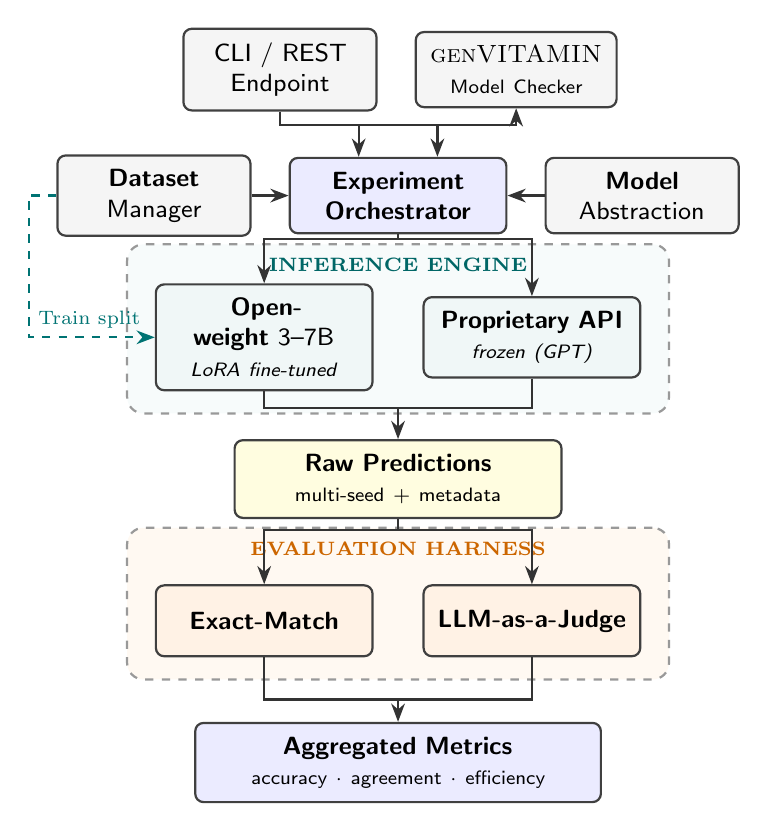
\begin{tikzpicture}[
    font=\small\sffamily,
    >=Stealth,
    % Standard box styles
    box/.style={
        rectangle, draw=black!75, thick, rounded corners=3pt,
        align=center, fill=white, minimum height=9mm, inner sep=5pt
    },
    io/.style={box, fill=gray!8},
    core/.style={box, fill=blue!8},
    data/.style={box, fill=yellow!12},
    infer/.style={box, fill=teal!6},
    eval/.style={box, fill=orange!10},
    % Grouping box styles
    grp/.style={
        rectangle, draw=black!40, thick, dashed, rounded corners=6pt,
        inner xsep=10pt, inner ysep=8pt
    },
    % Arrow styles
    arr/.style={->, thick, draw=black!80},
    trainarr/.style={->, thick, dashed, draw=teal!90!black},
    line/.style={thick, draw=black!80}
]

% ==========================================
% NODES & PLACEMENT
% ==========================================

% --- Core Architecture (Level 1) ---
\node[core, text width=2.4cm] (orch) at (0, 3) {\textbf{Experiment}\\\textbf{Orchestrator}};
\node[io, text width=2.1cm] (dm) at (-3.1, 3) {\textbf{Dataset}\\Manager};
\node[io, text width=2.1cm] (mal) at (3.1, 3) {\textbf{Model}\\Abstraction};

% --- Inputs (Level 0) ---
% Positioned slightly inward to ensure downward lines cleanly avoid the DM/MAL boxes
\node[io, text width=2.1cm] (cli) at (-1.5, 4.6) {CLI / REST\\Endpoint};
\node[io, text width=2.2cm] (vit) at (1.5, 4.6) {\textsc{genVITAMIN}\\{\scriptsize Model Checker}};

% --- Inference Engine (Level 2) ---
\node[infer, text width=2.4cm] (local) at (-1.7, 1.2) {\textbf{Open-weight} 3--7B\\{\scriptsize \textit{LoRA fine-tuned}}};
\node[infer, text width=2.4cm] (cloud) at (1.7, 1.2) {\textbf{Proprietary API}\\{\scriptsize \textit{frozen (GPT)}}};

% --- Raw Predictions (Level 3) ---
\node[data, text width=3.8cm] (pred) at (0, -0.6) {\textbf{Raw Predictions}\\{\scriptsize multi-seed $+$ metadata}};

% --- Evaluation Harness (Level 4) ---
\node[eval, text width=2.4cm] (em) at (-1.7, -2.4) {\textbf{Exact-Match}};
\node[eval, text width=2.4cm] (judge) at (1.7, -2.4) {\textbf{LLM-as-a-Judge}};

% --- Final Output (Level 5) ---
\node[core, text width=4.8cm] (metrics) at (0, -4.2) {\textbf{Aggregated Metrics}\\{\scriptsize accuracy $\cdot$ agreement $\cdot$ efficiency}};

% ==========================================
% BACKGROUND GROUPINGS
% ==========================================
\begin{scope}[on background layer]
    % Inference Engine Group
    \coordinate (inf_top) at (0, 2.1);
    \node[grp, fill=teal!3, fit=(local)(cloud)(inf_top)] (inf_box) {};
    \node[below=2pt of inf_box.north, font=\bfseries\scriptsize\color{teal!80!black}] {INFERENCE ENGINE};

    % Evaluation Harness Group
    \coordinate (eval_top) at (0, -1.5);
    \node[grp, fill=orange!5, fit=(em)(judge)(eval_top)] (eval_box) {};
    \node[below=2pt of eval_box.north, font=\bfseries\scriptsize\color{orange!80!black}] {EVALUATION HARNESS};
\end{scope}

% ==========================================
% ROUTING & ARROWS
% ==========================================

% 1. Inputs to Orchestrator
\draw[arr] (cli.south) |- (0, 3.9) -| ([xshift=-0.5cm]orch.north);
\draw[<->, thick, draw=black!80] (vit.south) |- (0, 3.9) -| ([xshift=0.5cm]orch.north);

% 2. DM and MAL to Orchestrator
\draw[arr] (dm.east) -- (orch.west);
\draw[arr] (mal.west) -- (orch.east);

% 3. DM to Local Model (Train Split fine-tuning loop)
% Wraps cleanly around the outside left edge
\draw[trainarr] (dm.west) -- ++(-0.35, 0) |- (local.west) 
    node[pos=0.74, above, font=\scriptsize\color{teal!90!black}, inner sep=3pt] {Train split};

% 4. Orchestrator fork to Inference
\draw[line] (orch.south) -- (0, 2.45);
\draw[arr] (0, 2.45) -| (local.north);
\draw[arr] (0, 2.45) -| (cloud.north);

% 5. Inference merge to Predictions
\draw[line] (local.south) |- (0, 0.3);
\draw[line] (cloud.south) |- (0, 0.3);
\draw[arr] (0, 0.3) -- (pred.north);

% 6. Predictions fork to Evaluators
\draw[line] (pred.south) -- (0, -1.25);
\draw[arr] (0, -1.25) -| (em.north);
\draw[arr] (0, -1.25) -| (judge.north);

% 7. Evaluators merge to Metrics
\draw[line] (em.south) |- (0, -3.4);
\draw[line] (judge.south) |- (0, -3.4);
\draw[arr] (0, -3.4) -- (metrics.north);

\end{tikzpicture}%
}
\caption{The \texttt{nl2atl} architecture. A natural-language requirement (from the CLI, a REST endpoint, or the integrated \textsc{genVITAMIN} model checker) reaches the \emph{Experiment Orchestrator}, which draws stratified splits and exemplars from the \emph{Dataset Manager} and resolves models through the \emph{Model Abstraction Layer}. Inference is hybrid: open-weight $3$--$7$B models are LoRA fine-tuned and served locally (dashed arrow), while proprietary API models are used frozen, behind one interface. Each generation is stored as a multi-seed raw prediction and scored by two independent evaluators (exact match and an LLM-as-a-judge) before aggregation into accuracy, agreement, and efficiency metrics.}
\label{fig:tool_pipeline}
\end{figure}

\subsection{Architecture}
Requests enter through a command-line interface or a REST endpoint and reach an \textbf{Experiment Orchestrator}. It draws data from a \textbf{Dataset Manager} (which produces deterministic, stratified train/validation/test partitions and holds the curated few-shot exemplars out of every split, so no prompting example leaks into evaluation) and resolves models through a \textbf{Model Abstraction Layer}, a declarative registry mapping a short model key to its provider, checkpoint, decoding parameters, and fine-tuning targets. The backing \textbf{Inference Engine} serves local open-weight checkpoints and cloud endpoints under one calling convention; because fine-tuning depends on initialization, each fine-tuned configuration is repeated over several seeds, while greedy decoding keeps run-to-run variation attributable to training rather than sampling. Every generation is stored as a \emph{raw prediction} with its metadata (latency, token counts, decoding configuration) before any scoring, and two evaluators then consume it: an \textbf{Exact-Match Evaluator} for normalized syntactic comparison and an \textbf{LLM-as-a-Judge} for meaning when surface forms diverge. Decoupling inference from evaluation, and applying the same two-tier scoring to local and cloud predictions alike, ensures that observed differences reflect model capability rather than the harness.

\subsection{Prompting and Output Parsing}
\label{subsec:prompting}
The translation target is pinned by a system prompt that fixes the ATL/ATL$^\ast$ surface syntax (the coalition modality $\langle\!\langle A \rangle\!\rangle$, the temporal operators $X$, $F$, $G$, and $U$, the Boolean connectives, \textsc{PascalCase} agent names, and \texttt{snake\_case} atomic propositions) together with the scope convention that keeps the strategic operator separate from the temporal operator it governs, e.g.\ $\langle\!\langle \mathrm{Machine}\rangle\!\rangle\,G(\mathit{paid}\rightarrow \mathit{printed})$ rather than $\langle\!\langle \mathrm{Machine}\rangle\!\rangle(G\,\mathit{paid}\rightarrow \mathit{printed})$. It also states the intended treatment of each targeted ambiguity: repeat the recovered formula for VP ellipsis, share the right-peripheral objective across both conjuncts for Right Node Raising, and emit \emph{all} admissible readings (one per line) for quantifier-scope ambiguity, never fusing two distinct readings into one. The few-shot condition prepends a small curated pool of exemplars spanning these phenomena, held out of every split. Models emit plain text under greedy decoding; a parser then strips extraneous tokens and canonicalizes whitespace, letter case, and operator spelling, so that scoring compares formulas rather than incidental surface form. A requirement with several readings is stored as a set of gold formulas, and a prediction must reproduce the entire set to count as correct. The full system prompt and the curated few-shot exemplars are reproduced in the technical appendix.

\subsection{Hybrid Inference: Privacy and Capacity}
\label{subsec:hybrid}
Confidentiality of requirements is a central concern in industrial formal methods, so the framework treats local open-weight inference as a primary path: checkpoints are fine-tuned with low-rank adapters~\cite{hu2022lora}, with $4$-bit QLoRA quantization~\cite{dettmers2023qlora} for the larger $7$B models, enabling domain specialization entirely on-premises, with no requirement leaving the air-gapped environment. The same interface targets Azure OpenAI endpoints when data sensitivity permits, letting practitioners trade data sovereignty against reasoning capacity without altering the pipeline.

\subsection{Scalability and Reproducibility}
\label{subsec:scale}
The framework targets large parameter sweeps over models, prompting conditions, and seeds: each $(\text{model}, \text{condition}, \text{split})$ cell is an independent unit of work dispatched to a SLURM-managed GPU cluster. To separate genuine capability from initialization noise, the orchestrator \emph{decouples} the data-split seed from the training seed and supports two protocols: a single \emph{canonical} stratified split, identical across models, used for the headline numbers reported here, and an optional stratified $k$-fold cross-validation mode, with shared folds, for estimating split-induced variance. Aggregation runs on the appropriate axis (over seeds or folds), yielding means with dispersion rather than single-point estimates.

\subsection{Model-Checker Integration}
\label{subsec:integration}
The practical value of a translation depends on its usability inside a verification workflow. We therefore connect \texttt{nl2atl} to \textsc{genVITAMIN}, an established model checker for strategic logics~\cite{DBLP:conf/ifaamas/0001M25}, so designers can express constraints in natural language and obtain formulas that are immediately parsed and verified (a screenshot is provided in the technical appendix). The integration is decoupled and dual-service: the verification backend manages the model-checking environment, while translation runs as a FastAPI microservice exposing a \texttt{/generate} endpoint that takes the requirement, a model key, and prompting flags (few-shot, maximum new tokens, and an optional fine-tuned adapter). A non-destructive patch installs a thin client so that ATL requests are routed to the translation service first and transparently fall back to the checker's native generation whenever the service is unavailable or returns an ill-formed result. Because the emitted formulas are parsed by the same front-end used for verification, only well-formed specifications enter model checking, giving immediate syntactic validation of model output.
\section{Evaluation Protocol}
\label{sec:evaluation}
We evaluate translations with a layered protocol that moves from strict syntax, to meaning, to the reliability of the evaluation itself, and finally to deployment efficiency. Every metric below is reported as a mean over independent runs rather than a single measurement.

\subsection{Multi-Seed Aggregation}
LLM decoding and fine-tuning are sensitive to initialization, so each fine-tuned configuration is run over several training seeds on the canonical split, and accuracy is reported as the seed mean together with a $95\%$ confidence interval. This makes the headline numbers stable estimates of capability rather than artifacts of a single favorable run.

\subsection{Exact Match and Meaning}
\noindent\textbf{Exact match.} Predictions are first compared to the reference under a normalization that removes purely surface differences: whitespace and letter case are normalized, logical operators are mapped to a canonical ASCII form (e.g.\ $\land,\lor,\neg,\to$), and the spelling of coalition names inside $\langle\!\langle\cdot\rangle\!\rangle$ is normalized while propositions are left intact, so that a non-semantic agent renaming is not penalized but a genuine lexical change still counts as a miss. Because a single requirement may admit several jointly required readings (for instance under quantifier-scope ambiguity), exact match demands that \emph{all} gold formulas be produced, not merely one of them. This deterministic check is the syntactic-precision baseline.

\noindent\textbf{LLM-as-a-judge.} A prediction that is \emph{not} an exact match is forwarded to an LLM-as-a-judge, which decides strategic and temporal equivalence to the reference and returns a structured verdict (a \texttt{correct} label and a free-text rationale). To avoid depending on any single model, we benchmark \emph{six} independent LLM judges (DeepSeek-V3.2, GPT-4.1, GPT-5.2, GPT-5.4, and the open-weight Gemma-2-27B and Llama-3.3-70B) under one fixed prompt (version~v1.4), whose adjudication rubric and calibration examples are reproduced in the technical appendix, and validate each against the expert audit below. Headline accuracy is reported under the single most human-aligned judge (the open-weight Llama-3.3-70B), which is moreover \emph{not} among the evaluated systems and so never grades its own outputs. Judge decisions are cached per judge identity, so the same judge is never queried twice on an identical triple, while the judges always remain independent. Reported accuracy is therefore the exact-match rate plus the judge-recovered fraction, a decomposition we state explicitly.

\noindent\textbf{Why an LLM judge rather than formal equivalence.} One might instead decide semantic equivalence of two ATL/ATL$^\ast$ formulas over concurrent game structures, but this is ill-posed here: the atomic propositions and agent names are grounded in the natural-language request rather than in a fixed game structure, so there is no shared model over which to evaluate satisfaction, and a faithful prediction may use a differently named but corresponding proposition or coalition; equivalence for ATL$^\ast$ is also computationally heavy. The judge therefore targets the appropriate notion: whether the prediction preserves the \emph{strategic-temporal intent} of the reference (coalition attribution, the strategic modality and its polarity, the temporal operators, and the scope relations among them) rather than verbatim form, requiring that all admissible readings appear for requirements with multiple readings. We treat these verdicts as estimates and validate them against human judgment next.

\subsection{Reliability of the Evaluation}
\noindent\textbf{Inter-rater agreement.} To quantify how trustworthy the automatic verdicts are, we compute pairwise Cohen's $\kappa$, Fleiss' $\kappa$, and Krippendorff's $\alpha$ across judges. Agreement is measured \emph{only} over items that actually reach the judges: deterministic verdicts---exact matches, and empty or unmatched predictions scored as incorrect without an LLM call---are excluded, since including them would trivially inflate agreement.

\noindent\textbf{Human validation.} An expert audit provides ground truth for the judges themselves. A stratified sample of $600$ items---deliberately over-representing items on which the judges disagree---is labeled independently by two expert annotators (inter-annotator agreement $99.5\%$, Cohen's $\kappa=0.99$). The annotators then deliberated over their three initial disagreements and reached agreement on two of them; the third resisted consensus and is retained as a genuine unresolved disagreement, excluded from the human-as-reference comparison and leaving $599$ consensus labels. On both reconciled cases the annotators concluded that the prediction \emph{was} faithful, overturning the stricter initial reading that the automated judges had echoed, so here the human audit corrects an over-strict tendency shared by the LLM judges rather than merely confirming them. The single remaining case sits on the boundary of strategic--temporal equivalence, an inherent limit that no equivalence-labeling protocol, human or automated, can fully avoid. The consensus labels both measure how closely each judge tracks human judgment and produce a robustness ranking in which human labels \emph{override} the judges wherever an item was audited. Because the judges track human judgment unevenly, we report headline accuracy under the most human-aligned judge alone, with two cross-checks for robustness: a conservative mean over DeepSeek-V3.2 and the stricter GPT-5.2 (both external to the evaluated systems), and a mean over all six judges.

\subsection{Efficiency}
We characterize deployment efficiency through the accuracy--latency trade-off rather than a single scalar: for every system we report mean per-example latency alongside accuracy and identify the Pareto frontier, the systems for which no alternative is simultaneously faster and more accurate. We avoid monetary cost models, since token prices and amortized GPU-hour rates are provider- and hardware-specific, whereas accuracy and latency are measured directly. One caveat applies to latency: cloud models are timed end-to-end over the network, so their latency is comparable within the local group but only indicative across the API/local boundary, while accuracy remains comparable throughout.

\subsection{Significance and Transparency}
To establish whether the leading system is genuinely ahead of its closest competitors, we compare systems on shared items with a paired bootstrap confidence interval and a randomization test, rather than the marginal accuracy gap alone. We also disclose every provider content-filter event: the few inputs rejected by the cloud safety filter (at generation or judging time) count as incorrect in the reported accuracy, are listed explicitly, and the ranking is recomputed with them excluded to confirm that the conclusions do not depend on them.



%\paragraph{Architectural Setup.}
%All experiments were conducted using the \texttt{nl2atl} framework implemented in Python~3.10 and executed on a Linux-based environment. The inference backend is built on a modular architecture supporting both local open-weight models and cloud-based APIs, with local inference executed on GPU-enabled nodes equipped with NVIDIA accelerators. Model orchestration, data handling, and evaluation pipelines are implemented using standard scientific Python libraries, while large-scale experimental runs are managed via SLURM on a high-performance computing cluster. The model-checking and syntactic validation of generated ATL/ATL$^\ast$ formulas are performed using the \textsc{VITAMIN} verification tool, ensuring that all evaluated outputs are compatible with an existing strategic model-checking pipeline.



%\subsection{Use Case Scenario} 
%Bob is an engineer working with a CGS in which he must guarantee a winning outcome. To reason about such strategic objectives, he requires a formalism for strategic reasoning with semantics that enforce victory, such as ATL. However, Bob is not an expert in formal logics and lacks the knowledge required to construct well-formed ATL formulas. Therefore, he seeks assistance from an LLM to translate his informal specifications into a formally correct verifiable goal. "In every interaction, the user can, if he is in coalition with the ticket machine, obtain a ticket after paying for it."


%\paragraph{Discussion.}
%This case study illustrates how the specifications produced by our NL-to-ATL$^*$ translator can be grounded and evaluated in simulation-based environments using a finite-trace interpretation of a strategic logic fragment. While this evaluation does not constitute ATL$^*$ model checking in the classical sense, it provides a principled and reproducible methodology for assessing strategic requirements in settings where full game-theoretic models are unavailable. We view this as a complementary validation approach that extends the practical applicability of NL-driven formal specification frameworks to realistic multi-agent simulations.





\section{Experiments}
\label{sec:experiments}

\begin{table}[t]
\centering
\small
\setlength{\tabcolsep}{4pt}
\begin{tabular}{@{}llcccc@{}}
\toprule
& & \multicolumn{2}{c}{\textbf{Baseline}} & \multicolumn{2}{c}{\textbf{Fine-tuned}} \\
\cmidrule(lr){3-4}\cmidrule(lr){5-6}
\textbf{Model} & \textbf{Size} & ZS & FS & ZS & FS \\
\midrule
\multicolumn{6}{@{}l}{\textit{Proprietary (Azure API)}}\\
gpt-4.1        & API  & 0.611 & 0.843 & --    & --    \\
gpt-5.4        & API  & \textbf{0.694} & \textbf{0.856} & --    & --    \\
\midrule
\multicolumn{6}{@{}l}{\textit{Open-weight (local)}}\\
mistral-7b     & 7B   & 0.239 & 0.349 & 0.762 & 0.766 \\
qwen-3b        & 3B   & 0.151 & 0.367 & 0.778 & 0.801 \\
phi3           & 3.8B & 0.275 & 0.417 & 0.800 & 0.818 \\
qwen-coder-7b  & 7B   & 0.298 & 0.463 & \textbf{0.839} & \textbf{0.844} \\
\bottomrule
\end{tabular}
\caption{\textbf{Primary results.} Semantic accuracy under the most human-aligned judge---the open-weight \textsc{Llama-3.3-70B}, which tracks the expert audit best among six candidates (Cohen's $\kappa=0.59$; cf.\ Table~\ref{tab:judge_reliability})---reported as the seed mean. ZS/FS denote zero-/few-shot prompting; fine-tuning is available only for the open-weight models; best per column in bold; fine-tuned values are means over three training seeds. Under this judge the strongest few-shot proprietary baseline (\textsc{gpt-5.4}, $0.856$) and the top fine-tuned open-weight system (\textsc{qwen-coder-7b}, $0.844$) are statistically tied within the $n{=}218$ sampling noise, so small fine-tuned open-weight models \emph{match} much larger few-shot proprietary ones. A conservative six-judge cross-check appears in the technical appendix.}
\label{tab:accuracy}
\end{table}

We report an empirical study on the held-out test split using the protocol of Section~\ref{sec:evaluation}. The questions are practical: can LLMs translate natural language into strategic temporal logic reliably enough to feed a verifier, and how do locally deployable open-weight models compare with proprietary baselines?

\paragraph{Setting.}
We evaluate six models across four conditions, yielding $20$ model--condition systems (fine-tuning applies only to the four open-weight models). Two proprietary Azure OpenAI models, \textsc{gpt-4.1} and \textsc{gpt-5.4}, are run zero- and few-shot as strong baselines: being closed-weight, they cannot be adapted within our on-premises setting, and the modest in-domain data makes API-side fine-tuning at their scale impractical, so they serve as strong \emph{few-shot} reference points. Our central comparison thus contrasts in-domain fine-tuning of small open-weight models with few-shot prompting of much larger proprietary ones, rather than model class alone. Four open-weight models---\textsc{mistral-7b}, \textsc{qwen-3b}, \textsc{phi3} (Phi-3.5-mini), and \textsc{qwen-coder-7b}---are run as baselines and after LoRA fine-tuning, in both prompting conditions. All systems share identical prompt templates, few-shot exemplars, and decoding (one greedy decode per query, with no chain-of-thought, self-consistency, or parser-feedback/self-repair scaffolding for any model), with local fine-tuning and inference on NVIDIA A100 GPUs, so the comparison isolates in-domain fine-tuning versus few-shot prompting rather than inference-time engineering applied unevenly. The parser canonicalizes surface form identically before scoring, and the tool's parser-validated fallback (Section~\ref{subsec:integration}) is a model-agnostic deployment feature held out of this controlled comparison; the proprietary baselines thus receive the same best-effort prompting as the open-weight systems, and the reported accuracies are a conservative floor that such scaffolding could lift for all alike. Of the $1100$ instances, the $7$ curated few-shot exemplars are held out of every split; the remaining $1093$ are partitioned by a stratified $70/10/20$ split into $765$ training, $110$ validation, and $218$ test examples. Each fine-tuned configuration is repeated over three training seeds, and every prediction is scored by six LLM judges (DeepSeek-V3.2, GPT-4.1, GPT-5.2, GPT-5.4, and the open-weight Gemma-2-27B and Llama-3.3-70B) plus an expert human audit on a stratified subsample, for $4{,}279$ items with multiple judge verdicts.

\paragraph{Fine-tuning versus few-shot baselines.}
Table~\ref{tab:accuracy} reports semantic accuracy by model and condition under the most human-aligned judge. The top is a statistically tied cluster: the strongest few-shot proprietary baseline, \textsc{gpt-5.4} few-shot ($0.856$), and the best fine-tuned open-weight system, \textsc{qwen-coder-7b} few-shot ($0.844$), differ by only $0.012$---within the $n{=}218$ sampling noise---so small fine-tuned open-weight models \emph{match} much larger few-shot proprietary ones. Fine-tuning is the dominant factor for the open-weight models: it lifts \textsc{phi3} from $0.417$ to $0.818$ in the few-shot setting and moves every open-weight model from weak zero-shot baselines (as low as $0.151$) into the $0.76$--$0.84$ band. Few-shot prompting helps throughout, but its benefit is largest for the untuned baselines and shrinks after fine-tuning, so task adaptation, rather than scale alone, drives open-weight performance: the $3$--$7$B fine-tuned models reach the level of much larger \emph{few-shot} proprietary systems. These gains come from fine-tuning on the $765$-instance training split, augmented twofold by templated paraphrasing of the input (synonym substitutions for temporal and strategic phrasings that leave the gold formula unchanged), applied to training only, so validation and test are never augmented; modest in-domain supervision thus suffices to specialize a small model to ATL/ATL$^\ast$. The $95\%$ seed confidence intervals for the top systems are narrow (about $\pm0.02$; see the six-judge robustness check in the technical appendix), but they capture only training-seed variation at the fixed canonical split and \emph{not} test-set sampling variance, which at $n{=}218$ items is on the order of $\pm0.06$; the seed intervals are therefore a lower bound, and a stratified $k$-fold sweep, which our framework supports, would estimate the split component directly and is left to future runs.

\paragraph{Exact match versus meaning.}
We decompose accuracy under the most human-aligned judge into a deterministic exact-match floor and the fraction the LLM judge recovers (the appendix gives the full breakdown for the headline systems under the same judge). The gap between syntactic and meaning-level scoring is large and uneven, and widest for the proprietary baselines. For \textsc{gpt-5.4} zero-shot, exact match yields only $0.213$ of the $0.694$ accuracy: roughly $69\%$ of correct answers are syntactically distinct from the reference yet strategically equivalent; for \textsc{gpt-4.1} few-shot the judge-recovered share is $46\%$. It is smaller for the strongest fine-tuned systems ($23$--$29\%$), whose outputs more often match the reference surface form, but never negligible. Purely syntactic metrics therefore systematically understate translation quality, especially on underspecified requirements.

\paragraph{Statistical significance.}
A paired analysis on shared items confirms a tight top cluster and shows that the comparison with the proprietary baselines is itself judge-dependent, in the direction our judge-reliability analysis predicts. The fine-tuned \textsc{phi3} and \textsc{qwen-coder-7b} systems (few- and zero-shot) are mutually indistinguishable (pairwise differences $\le 0.024$ under the six-judge mean, within the $n{=}218$ sampling noise) and far above the untuned open-weight baselines. Against \textsc{gpt-5.4} few-shot the paired difference changes sign with the judge: under the most human-aligned judge of Table~\ref{tab:accuracy} the two are statistically level (\textsc{qwen-coder-7b} few-shot $\Delta=-0.009$, randomization $p=0.71$), whereas under the six-judge mean the open-weight systems edge ahead by a small margin (\textsc{qwen-coder-7b} $\Delta=0.052$, paired bootstrap $95\%$ CI $[0.004,0.102]$, $p=0.03$; \textsc{phi3} $\Delta=0.048$, $p=0.03$). That swing is precisely the artifact documented above (the stricter judges penalise the proprietary baselines' faithful input-grounded paraphrases more heavily, while the most human-aligned judge credits them), so we read the generation comparison as \emph{parity}: the fine-tuned open-weight systems are statistically level with the few-shot proprietary baselines under the most reliable judge, and the small lead that appears under stricter scoring reflects judge over-strictness rather than a true quality gap.

\paragraph{Judge reliability.}
{\sloppy\setlength{\emergencystretch}{3em}
Table~\ref{tab:judge_reliability} summarizes inter-rater reliability, and it carries our most striking result: \emph{judge quality runs opposite to generator strength}. The six LLM judges agree only moderately with one another (mean pairwise Cohen's $\kappa=0.49$) and track the human audit very unevenly. The strongest, most recent proprietary models are the \emph{worst} judges---\textsc{gpt-5.4}, the top few-shot \emph{generator} in Table~\ref{tab:accuracy}, manages only $\kappa=0.24$ against humans and \textsc{gpt-5.2} worse still ($\kappa=0.16$)---whereas the best judge by a wide margin is the open-weight \textsc{Llama-3.3-70B} ($\kappa=0.59$, $81.8\%$ agreement), ahead of \textsc{DeepSeek-V3.2} ($0.46$) and \textsc{gpt-4.1} ($0.44$). The cause is systematic over-strictness on predicate \emph{aliasing}: on $1167$ items both strict proprietary judges (\textsc{gpt-5.4} and \textsc{gpt-5.2}) rejected a prediction that \textsc{Llama-3.3-70B} accepted---and on the audited subset the human experts sided with \textsc{Llama} over them $160$ to $26$---while there is \emph{not a single} item where \textsc{Llama} rejected a prediction both of these judges accepted. Almost all such cases merely rename an atomic proposition to an input-grounded paraphrase (\texttt{discharged}\,$\to$\,\texttt{patient\_discharged}, \texttt{error}\,$\to$\,\texttt{error\_state}) while preserving every coalition, temporal operator and connective, which the rubric instructs judges to accept but \textsc{gpt-5.4}/\textsc{gpt-5.2} reject as ``not a clearly grounded alias''. This strictness is not self-serving: \textsc{gpt-5.4} as a judge marks down the \emph{proprietary} generations too, scoring its own few-shot output at $0.634$ where \textsc{Llama} gives $0.856$, so the strong proprietary models penalise even their own family and only the open-weight judge recovers their true accuracy. We therefore report headline accuracy under \textsc{Llama-3.3-70B}, the most human-aligned judge and itself external to the evaluated systems. The choice is robust: under the conservative six-judge mean the fine-tuned open-weight systems even \emph{lead} the proprietary baselines, and when human labels override the judges wherever an item was audited the top cluster is unchanged; only the \emph{size} of the open-weight margin moves with the judge, shrinking to a tie under the human-aligned \textsc{Llama}.\par}

\begin{table}[t]
\centering
\small
\begin{tabular}{@{}lccc@{}}
\toprule
\textbf{Judge vs.\ human} & $n$ & \textbf{Agr.} & \textbf{Cohen's} $\kappa$ \\
\midrule
\textbf{Llama-3.3-70B} & $598$ & $\mathbf{81.8\%}$ & $\mathbf{0.59}$~(mod.) \\
DeepSeek-V3.2 & $598$ & $73.7\%$ & $0.46$~(mod.) \\
GPT-4.1       & $598$ & $72.7\%$ & $0.44$~(mod.) \\
Gemma-2-27B   & $598$ & $59.4\%$ & $0.25$~(fair) \\
GPT-5.4       & $598$ & $56.9\%$ & $0.24$~(fair) \\
GPT-5.2       & $598$ & $50.7\%$ & $0.16$~(slight) \\
\bottomrule
\end{tabular}
\caption{\textbf{Judge reliability against the human audit.} Agreement of each of the six LLM judges with the consensus expert labels on the audited items; ``Agr.''\ is the exact label-match rate and the $\kappa$ interpretation follows Landis--Koch. Among the judges themselves, mean pairwise Cohen's $\kappa=0.49$ (range $0.19$--$0.62$; $65$--$91\%$ raw agreement); adding the human as a seventh rater gives Fleiss' $\kappa=0.42$. The open-weight \textsc{Llama-3.3-70B} tracks humans most closely---well ahead of the substantially more recent and more capable \textsc{gpt-5.4} and \textsc{gpt-5.2}---so it serves as the headline judge, illustrating that judge quality runs opposite to generator quality. Each judge is compared against the $598$ audited predictions that carry a consensus expert label; one further audited prediction, on which the annotators reached no consensus, is excluded (its case appears in the technical appendix).}
\label{tab:judge_reliability}
\end{table}

\paragraph{Efficiency.}
We characterize efficiency through the accuracy--latency trade-off, plotted in the technical appendix. The two fastest fine-tuned open-weight systems are also among the most accurate: few-shot \textsc{qwen-3b} ($1567$\,ms) and \textsc{phi3} ($1681$\,ms), both faster than the proprietary baselines \textsc{gpt-4.1} ($1979$\,ms) and \textsc{gpt-5.4} ($2538$\,ms); few-shot \textsc{qwen-coder-7b} reaches the top open-weight accuracy ($3338$\,ms), and fine-tuned \textsc{mistral-7b} is slowest ($4460$\,ms). The accuracy--latency frontier is therefore shared between the fast fine-tuned open-weight systems and the marginally more accurate few-shot proprietary baselines; since the open-weight models match them on accuracy (Table~\ref{tab:accuracy}) while running on-premises and, for the fastest two, at lower latency, they remain preferable for local deployment. The proprietary latencies are network-timed and only indicative across the API/local boundary.

\paragraph{Robustness to content filtering.}
The Azure safety filter blocked only two inputs (a Shakespeare quotation and one other), counted as incorrect; excluding them leaves every system's rank unchanged, so no conclusion hinges on provider-side filtering.

\paragraph{Error analysis by ambiguity type.}
The failure modes cluster by linguistic phenomenon. The dominant errors of the \emph{untuned} open-weight models are syntactic: predictions borrow CTL-style path quantifiers (e.g.\ \texttt{AF\,p}) for the coalition modality, introduce first-order quantifiers and variables foreign to ATL/ATL$^\ast$, or emit malformed coalitions, all rejected by both exact match and the judges. Fine-tuning largely removes these gross errors, accounting for the steep zero-shot-to-fine-tuned jump. The residual errors concentrate on the ambiguity families: under quantifier-scope ambiguity the models most often \emph{collapse} the distributive and collective readings into one formula or return only one of the two required; under VP ellipsis and Right Node Raising they fail to \emph{reconstruct} the shared objective for the second agent; and dislocation occasionally yields a mis-attributed coalition. Temporal-operator substitutions (e.g.\ \texttt{U} for \texttt{F}) and spurious or dropped negations occur across categories but are rare once a model is fine-tuned. These patterns track the benchmark's design intent: once surface syntax is mastered, the discriminating difficulty is recovering the intended \emph{scope} and \emph{distribution} of strategic ability, not lexical translation. The technical appendix makes this quantitative on the $31$ multi-reading (QSA) and $187$ single-reading test items (a re-aggregation of existing verdicts, no new labels). Single-reading accuracy is uniformly high ($0.85$--$0.88$), but every system drops sharply on the multi-reading slice, which remains the hardest phenomenon for all of them. Here no model class dominates: the strongest few-shot proprietary baseline (\textsc{gpt-5.4}, $0.68$) and the best fine-tuned open-weight model (\textsc{qwen-coder-7b}, $0.63$) are comparable, while the smaller fine-tuned models lag (\textsc{qwen-3b} $0.33$, \textsc{mistral-7b} $0.27$); with only $31$ QSA items these differences are within noise (binomial $95\%$ CI $\approx\pm0.17$), so we read the slice as a qualitative contrast rather than a ranking. Under the strictest judges the proprietary baselines instead collapse on this slice, an artifact of their over-strict rejection of input-grounded predicate paraphrases (documented in our judge-reliability analysis) rather than a failure to emit both readings, and one the human-aligned headline judge does not share.

\paragraph{Discussion.}
Taken together, our experiments show that in-domain fine-tuning of small open-weight models translates strategic requirements as accurately as strong few-shot proprietary baselines while keeping requirements on-premises; that open-weight models also make the most reliable automatic \emph{judges} of these translations, whereas the strongest proprietary models judge worst by over-rejecting faithful paraphrases; and that exact match alone is an inadequate metric. Complete tables, the training and decoding configuration, the computing infrastructure, and a reproducibility checklist appear in the technical appendix and supplementary material.
\section{Conclusions}
\label{sec:conclusions}

We introduced an open-weight, open-source framework for translating natural-language strategic requirements into well-formed ATL/ATL$^\ast$ specifications. Three contributions support it: an expert-authored dataset of $1100$ instances spanning simple requirements and five ambiguity families (right and left dislocation, VP ellipsis, Right Node Raising, and quantifier scope ambiguity), balanced over the ATL/ATL$^\ast$ temporal operators and reusable as a benchmark; a hybrid framework running both cloud APIs and local open-weight models with LoRA fine-tuning; and a multi-faceted evaluation protocol coupling normalized exact match with a human-validated LLM-as-a-judge. Our experiments show that in-domain fine-tuning of small, locally deployable open-weight models ($3$--$7$B) translates strategic requirements as accurately as strong few-shot proprietary baselines under the most human-aligned judge; that exact match alone understates quality, since faithful translations often differ syntactically from the reference; and that the automatic judges must themselves be validated, since judge reliability runs opposite to generator capability---the open-weight Llama-3.3-70B is the most human-aligned judge, while the strongest, most recent proprietary models are the least reliable, over-rejecting faithful paraphrases even of their own generations. Finally, the translations plug directly into \textsc{genVITAMIN}, an existing strategic model checker, illustrating a practical deployment path.



\paragraph{Limitations.}
Several limitations qualify these results. The benchmark, although expert-validated, is curated rather than drawn from deployed industrial requirements, and is English-only; transfer to in-the-wild specifications and other languages remains to be demonstrated. We target ATL/ATL$^\ast$, so requirements involving knowledge, beliefs, or the more expressive constructs of Strategy Logic lie outside the present scope. Semantic accuracy is measured by an LLM judge whose agreement with human experts---moderate even for the best-aligned judge---is imperfect, so the absolute numbers are best read as calibrated estimates rather than exact rates; we mitigate this with multiple independent judges and a human-overridden ranking. Our reported confidence intervals, moreover, reflect training-seed variation at a single canonical split; with only $218$ test items, test-set resampling adds uncertainty of order $\pm0.06$ that these intervals do not capture, so they are best read as a lower bound---a stratified $k$-fold evaluation, supported by our framework, would tighten this estimate. Finally, equivalence is assessed by strategic-temporal intent rather than by formal model checking, and the reported cross-environment latencies are only indicative across the API/local boundary.

\paragraph{Future Work.}
Several directions for future work emerge. The main avenue concerns extending the framework to more powerful strategic formalisms, such as Strategy Logic and its fragments~\cite{DBLP:journals/tocl/MogaveroMPV14,DBLP:conf/aaai/CermakLM15,DBLP:conf/ijcai/BelardinelliJKM19} or epistemic variants of ATL~\cite{DBLP:journals/fuin/JamrogaH04,aminof2016prompt,jamroga2017reasoning}, enabling translation about knowledge, beliefs, and information flow in MAS. Moreover, the released dataset opens the door to training domain-specialized models potentially reducing reliance on post-hoc semantic validation.

%Future work will focus on interactive disambiguation, richer strategic formalisms, and deeper coupling between translation models and verification feedback.


\bibliography{bibliography}

\end{document}
